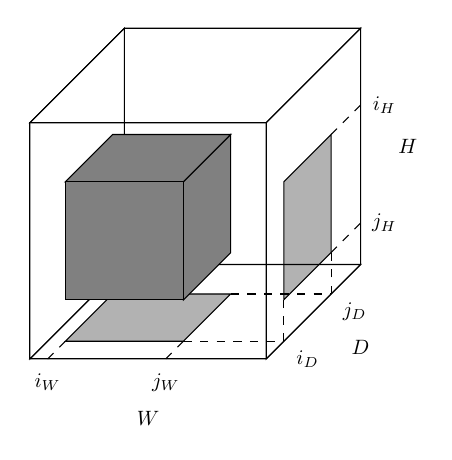
\begin{tikzpicture}[scale=.3, every node/.style={scale=0.75}]
	% \drawline#x1#y1#x2#y2#format
	\def\drawline#1#2#3#4#5{
		\draw[#5] (#1, #2) -- (#3, #4);
	}
	
	% \drawfacef#x#y#size#color#opacity#thickness
	\def\drawfacef#1#2#3#4#5#6{
		\filldraw[fill=#4, fill opacity=#5, #6] 
			(#1, #2) -- ++ (#3, 0) -- ++ (0,  #3) -- ++ (-#3, 0) -- cycle;
	}
	
	% \drawfaceh#x#y#size#color#opacity#thickness
	\def\drawfaceh#1#2#3#4#5#6{
		\filldraw[fill=#4, fill opacity=#5, #6] 
			(#1, #2) -- ++ (#3, 0) -- ++ (#3 * .4,  #3 * .4) -- ++ (-#3, 0) -- cycle;
	}
	
	% \drawfacev#x#y#size#color#opacity#thickness
	\def\drawfacev#1#2#3#4#5#6{
		\filldraw[fill=#4, fill opacity=#5, #6] 
			(#1, #2) -- ++ (#3 * .4,  #3 * .4) -- ++ (0, #3)  -- ++ (-#3 * .4, -#3 * .4) -- cycle;
	}
	
	% \drawcubid#x#y#size#color#opacity#thickness#showall
	\def\drawcubid#1#2#3#4#5#6#7{
		\ifx\\#7\\
			\drawfacev{#1}{#2}{#3}{#4}{#5}{#6} 						% L
			\drawfaceh{#1}{#2}{#3}{#4}{#5}{#6}  					% B
			\drawfacef{#1 + #3 * .4}{#2 + #3 * .4}{#3}{#4}{#5}{#6}	% R
		\fi
		\drawfacev{#1 + #3}{#2}{#3}{#4}{#5}{#6}  					% R
		\drawfaceh{#1}{#2 + #3}{#3}{#4}{#5}{#6}  					% T
		\drawfacef{#1}{#2}{#3}{#4}{#5}{#6} 							% F
	}
	
	
	% big cubid
	\drawcubid{0}{0}{10}{black}{0}{}{}
	
	% line, face and node
	\drawline{0.75}{0}{1.5}{0.75}{dashed}
	\drawline{5.75}{0}{6.5}{0.75}{dashed}
	\drawline{6.5}{0.75}{10.75}{0.75}{dashed}
	\drawline{8.5}{2.75}{12.75}{2.75}{dashed}
	\drawfaceh{1.5}{0.75}{5}{black}{0.3}{}
	
	\drawline{10.75}{0.75}{10.75}{2.5}{dashed}
	\drawline{12.75}{2.75}{12.75}{4.5}{dashed}
	\drawline{12.75}{4.5}{14}{5.75}{dashed}
	\drawline{12.75}{9.5}{14}{10.75}{dashed}
	\drawfacev{10.75}{2.5}{5}{black}{0.3}{}
	
	\node at (0.75, -1) {$i_W$};
	\node at (5.75, -1) {$j_W$};
	\node at (5, -2.5) {$W$};
	
	\node at (11.75, 0) {$i_D$};
	\node at (13.75, 2) {$j_D$};
	\node at (14, 0.5) {$D$};
	
	\node at (15, 10.75) {$i_H$};
	\node at (15, 5.75) {$j_H$};
	\node at (16, 9) {$H$};
	
	% small cuid
	\drawcubid{1.5}{2.5}{5}{gray}{1}{}{n}
\end{tikzpicture}